\documentclass{beamer}
\beamertemplatenavigationsymbolsempty
\usecolortheme{beaver}
\setbeamertemplate{blocks}[rounded=true, shadow=true]
\setbeamertemplate{footline}[page number]
%
\usepackage[utf8]{inputenc}
\usepackage[english,russian]{babel}
\usepackage{amssymb,amsfonts,amsmath,mathtext}
\usepackage{subfig}
\usepackage[all]{xy} % xy package for diagrams
\usepackage{array}
\usepackage{multicol} % many columns in slide
\usepackage{hyperref} % urls
\usepackage{hhline} %tables
\usepackage{comment} %comments
% Your figures are here:
\graphicspath{ {fig/} {../fig/} }

%----------------------------------------------------------------------------------------------------------

\title[\hbox to 56mm{Классификация траекторий физических систем}]{Классификация траекторий физических систем\\ с помощью лагранжевых нейронных сетей}
\author[А.\,И.~Богданов]{Александр Иванович Богданов}
\institute{Московский физико-технический институт}
\date{\footnotesize
\par\smallskip\emph{Курс:} Моя первая научная статья
\par\smallskip\emph{Эксперт:} В.\,В.~Стрижов
\par\smallskip\emph{Консультант:} С.\,К.~Панченко
\par\bigskip\small 2023}

%----------------------------------------------------------------------------------------------------------

\begin{document}

%----------------------------------------------------------------------------------------------------------

\begin{frame}

    \thispagestyle{empty}
    \maketitle
    
\end{frame}

%-----------------------------------------------------------------------------------------------------

\begin{frame}{Цель исследования}
    \begin{block}{Цель}
        Исследование методов классификации траекторий физических систем.
    \end{block}
    \begin{block}{Проблема}
        Стандартные методы классификации не учитывают физическую связь координат и динамики системы.
    \end{block}
    \begin{block}{Решение}
        Моделирование лагранжиана с помощью лагранжевых нейронных сетей с последующим использованием полученных коэффициентов в качестве признаковых описаний для определения вида движения.
    \end{block}
\end{frame}

%-----------------------------------------------------------------------------------------------------

\begin{frame}{Публикации по теме}
    \begin{itemize}
    
    \item Северилов Павел. Выбор оптимальной модели в задаче моделирования динамики физической системы. \url{https://github.com/severilov/master-thesis}.

    \item Miles Cranmer, Sam Greydanus, Stephan Hoyer, Peter Battaglia, David Spergel, and Shirley Ho. Lagrangian neural networks. arXiv preprint arXiv:2003.04630, 2020.

    \item Обработка датасета PAMAP2. https://github.com/andreasKyratzis/PAMAP2-Physical-Activity-Monitoring-Data-Analysis-and-ML/blob/master/pamap2.ipynb
  
    \end{itemize}
\end{frame}

%-----------------------------------------------------------------------------------------------------

\begin{frame}{Описание задачи классификации траекторий}

    Задана выборка с метками из $n$ траекторий
    $$\{ \mathcal{D}_j, z_j\}_{j=1}^n,$$ 

    \begin{itemize}

        \item[$\bullet$] $\mathcal{D}_j = \{ \mathbf{x}_i^{(j)}, \mathbf{y}_i^{(j)} \}_{i=1}^{m_j}$ ~-- $j$-ая траектория,

        \item[$\bullet$] $\mathbf{x}_i^{(j)} = (\mathbf{q}_i^{(j)}, \mathbf{\dot{q}}_i^{(j)})$ ~-- координаты $j$-ой траектории, 

        \item[$\bullet$] $\mathbf{y}_i^{(j)} = \mathbf{\dot{x}}_i^{(j)} = (\mathbf{\dot{q}}_i^{(j)}, \mathbf{\ddot{q}}_i^{(j)})$ ~-- динамика на $j$-ой траектории, 

        \item[$\bullet$] $\mathbf{q}_i^{(j)} \in \mathbb{R}^r$ ~-- вектор обобщенных координат,

        \item[$\bullet$] $r$ ~-- количество координат,

        \item[$\bullet$] $m_j$ ~-- длина $j$-ой траектории,

        \item[$\bullet$] $z_j$ ~-- метка $j$-ой траектории.
        
    \end{itemize}

\end{frame}    

%-----------------------------------------------------------------------------------------------------

\begin{frame}{Задача регрессии динамики физической системы}

    Регрессионная модель выбирается из класса нейронных сетей
    $$\mathbf{f_j} \colon (\mathbf{x}, \mathbf{w}) \to \mathbf{y}, \quad \mathbf{x} \in \mathbb{R}^{2 \times r}, \quad \mathbf{y} \in \mathbb{R}^{2 \times r},$$ 
    
    \begin{itemize}
    
            \item[$\bullet$] $\mathbf{w} \in \mathbb{W}$ ~-- параметры модели, 

            \item[$\bullet$] $\hat{\mathbf{y}}_i^{(j)} = \mathbf{f}_j (\mathbf{x}_i^{(j)}, \mathbf{w}) \in \mathbb{R}^{2 \times r}$ ~-- предсказанная динамика $j$-ой траектории,
        
            \item[$\bullet$] $\mathbf{X}_j = \bigcup_{i=1}^{m_j} \mathbf{x}_i^{(j)}$ ~-- матрица координат $j$-ой траектории,
            
            \item[$\bullet$] $\mathbf{Y}_j = \bigcup_{i=1}^{m_j} \mathbf{y}_i^{(j)}$ ~-- матрица динамики $j$-ой траектории,
            
            \item[$\bullet$] $\hat{\mathbf{Y}}_j = \bigcup_{i=1}^{m_j} \hat{\mathbf{y}}_i^{(j)}$ ~-- предсказанная матрица динамики $j$-ой траектории.
        
        \end{itemize}

        Задача минимизации квадратичной ошибки: 

        $$\mathcal{L}(\textbf{w}) = \mathcal{L}(\mathbf{w} | \mathbf{X}_j, \mathbf{Y}_j) = \| \hat{\mathbf{Y}}_j - \mathbf{Y}_j \|_2^2,$$
    
        $$\textbf{w}_j^* = \arg \min_{\mathbf{w} \in \mathbb{W}} \left( \mathcal{L}(\textbf{w}) \right).$$

\end{frame}

%----------------------------------------------------------------------------------------------------------

\begin{frame}{Задача классификации физических траекторий}

        Задача классификации:

        $$\{\textbf{w}^*_j, z_j\}_{j=1}^n,$$
        
        $\textbf{w}^*_j$ ~-- коэффициенты аппроксимированного лагранжиана $j$-ой траектории.
    
        Для ее решения используются различные методы классификации, среди которых: логистическая регрессия, ядерный метод с гауссовским ядром, случайный лес.


\end{frame}

%----------------------------------------------------------------------------------------------------------

\begin{frame}{Лагранжева динамика}

    Лагранжев формализм моделирует физическую систему с координатами траектории $\mathbf{x_t} = (\mathbf{q}, \dot{\mathbf{q}})$. Определяется функционал, называющийся действием:
    
    $$S=\int\limits_{t_0}^{t_1} L dt,$$
    показывающий путь, по которому координаты $\mathbf{x}_t$ пройдут из $\mathbf{x}_0$ в $\mathbf{x}_1$ в промежуток времени от $t_0$ до $t_1$. Путь минимизирует действие $S$, что приводит к уравнению Эйлера-Лагранжа

    $$\frac{d}{dt} \frac{\partial L}{\partial \dot{\mathbf{q}}} = \frac{\partial L}{\partial \mathbf{q}}$$

    Ускорение каждой компоненты системы $ \ddot{\mathbf{q}}$:

    $$\ddot{\mathbf{q}} = \left( \nabla_{\dot{\mathbf{q}}} \nabla_{\dot{\mathbf{q}}}^T L \right)^{-1} \left[ \nabla_{\mathbf{q}} L - \left( \nabla_{\dot{\mathbf{q}}} \nabla_{\mathbf{q}}^T L \right) \dot{\mathbf{q}} \right]$$


\end{frame}

%----------------------------------------------------------------------------------------------------------

\begin{frame}{Лагранжева нейронная сеть}

        Нейронная сеть
        $$f: \mathbf{X} = (\mathbf{q}, \mathbf{\dot{q}}) \rightarrow L.$$

        Схема работы LNN для задачи моделирования динамики системы

        \begin{figure}[H]
            \centering
            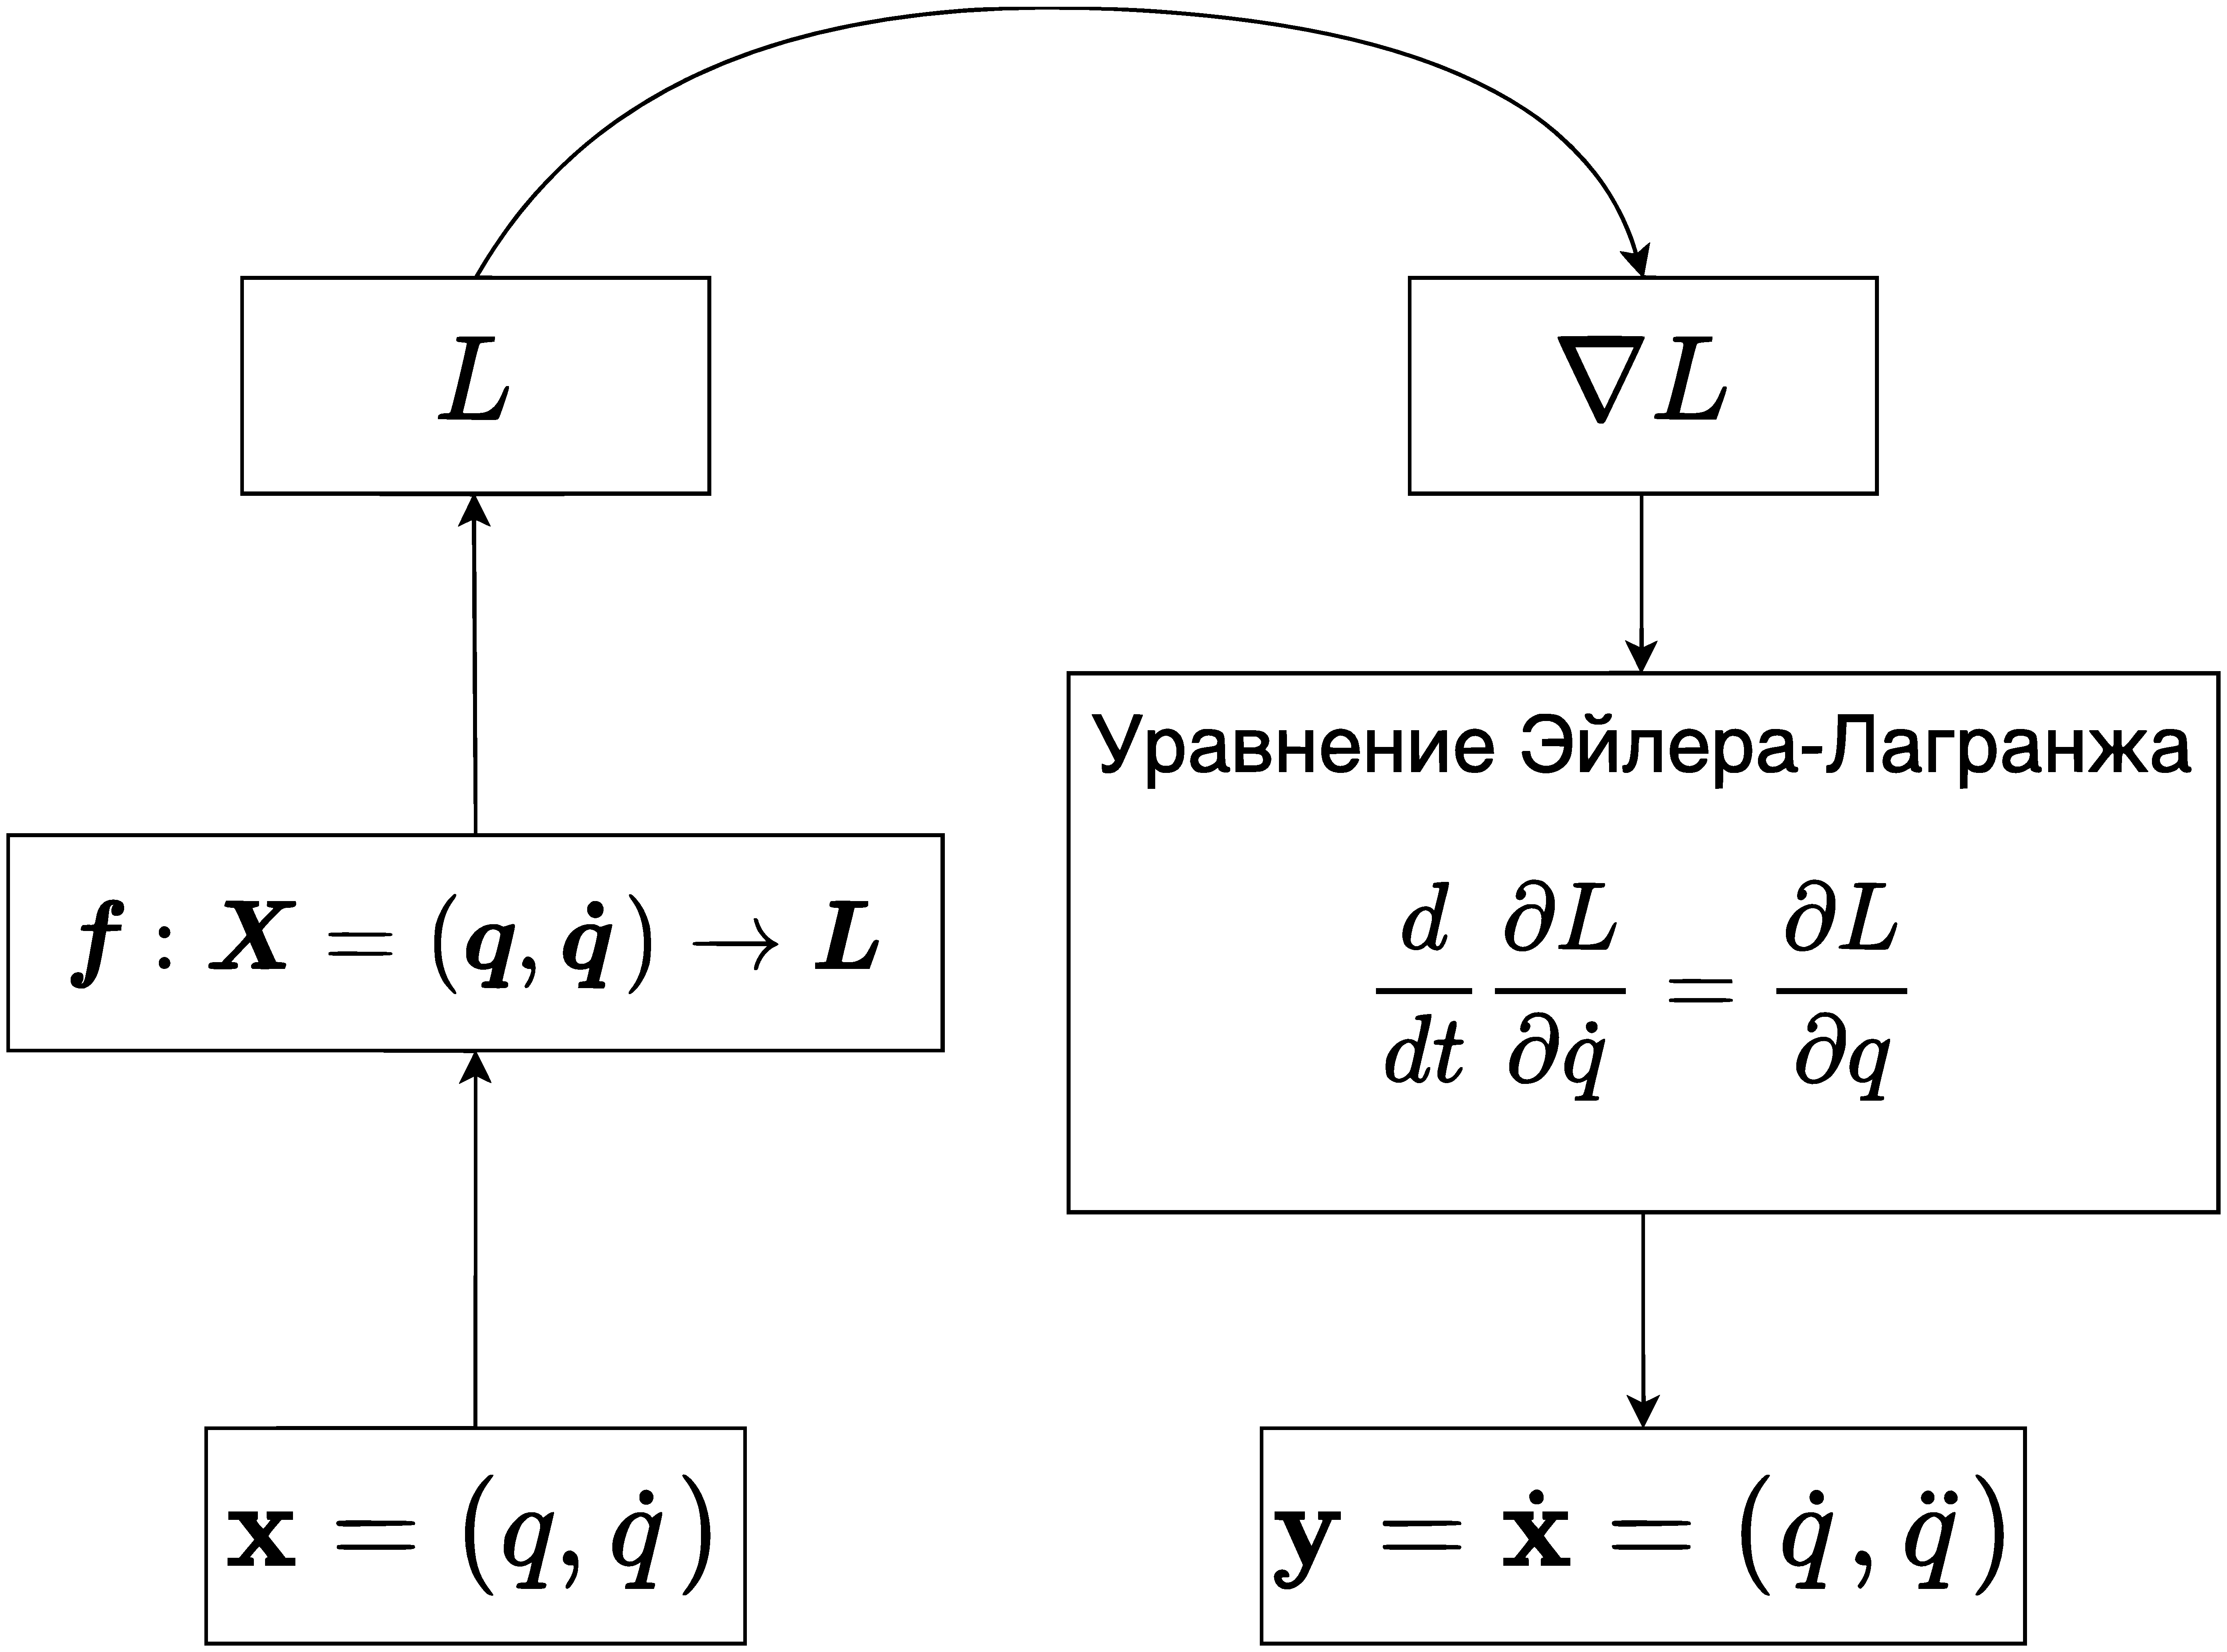
\includegraphics[width=0.7\textwidth]{LNN.eps}
        \end{figure}

        Необходимо параметризовать нейронной сетью лагранжиан $L$, получить выражение ограничения Эйлера-Лагранжа и обратно распространить ошибку через полученные ограничения.
    
\end{frame}

%----------------------------------------------------------------------------------------------------------

\begin{frame}{Подготовка данных}

    Для эксперимента используется датасет PAMAP2. Проблемы:
    
        \begin{itemize}
    
            \item Пропуски данных, связанные с тем, что датчик может пропустить такт. Для восстановления данных использовалась сплайн-интерполяция.

            \item Наличие скоростей и отсутствие ускорений и координат.
            
            Для получения ускорений используется аппроксимация 2-го порядка:
            $$f'(x_i) \approx \frac{f(x_{i + 1}) - f(x_{i - 1})}{2h}$$.

            Для получения координат используется метод Симпсона 3-го порядка аппроксимации::
            $$\int\limits_a^b f(x) dx \approx \frac{h}{3} \sum\limits_{k = 1}^{N - 1} \left( f(x_{k + 1} + 4f(x_k) + f(x_{k - 1}) \right)$$

        \end{itemize}

\end{frame}

%----------------------------------------------------------------------------------------------------------

\begin{frame}{Вычислительный эксперимент}

    Датасет:
    
    \begin{itemize}

        \item Акселерометры:
            \begin{itemize}

                \item На запястье рабочей руки

                \item На рабочей ноге

                \item На груди

            \end{itemize}

        \item Частота акселерометров: 100 Гц.
            
        \item Количество классов: K = 24.

    \end{itemize}

    Для эксперимента использовались данные с рабочей ноги и 4 класса, на которых движение этой ноги различно.
        
    Для каждого объекта из подвыборки строится лагранжиан. Затем параметры этого лагранжиана используются в качестве признаков. 

\end{frame}

%----------------------------------------------------------------------------------------------------------

\begin{frame}{Анализ ошибки}

    Распределение признаков:

        \begin{columns}[c]
        
            \column{0.6\textwidth}
                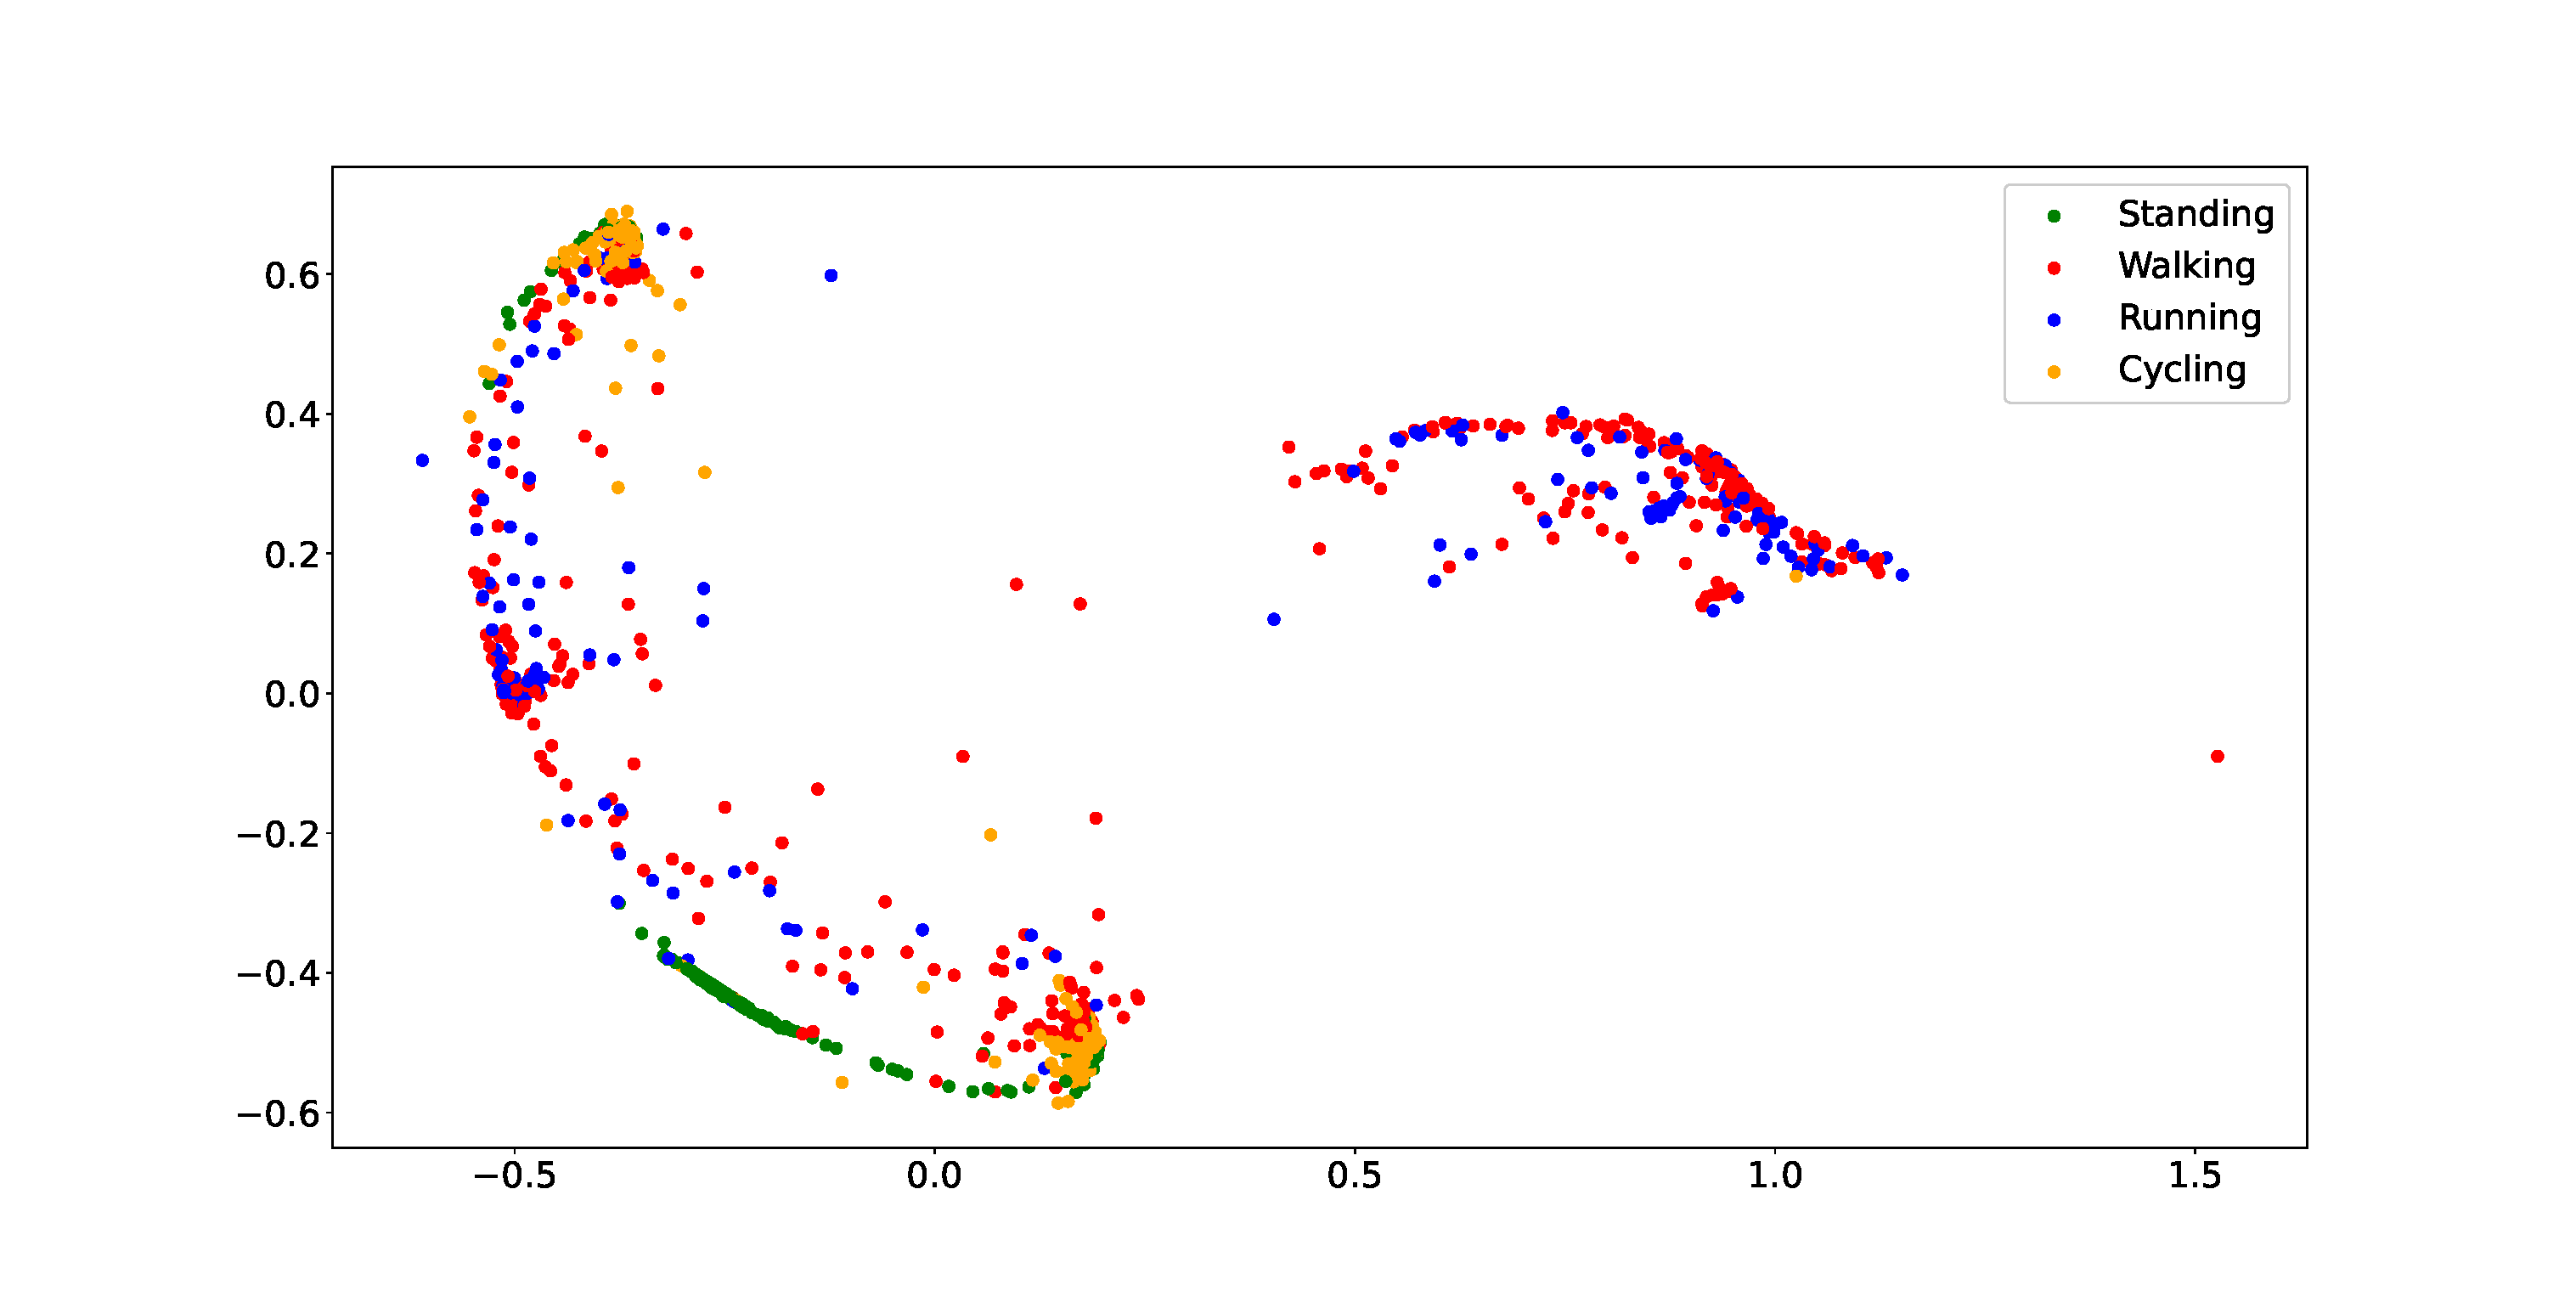
\includegraphics[width=1.1\textwidth]{Data_2D.eps}
                
            \column{0.6\textwidth}
                \centering
                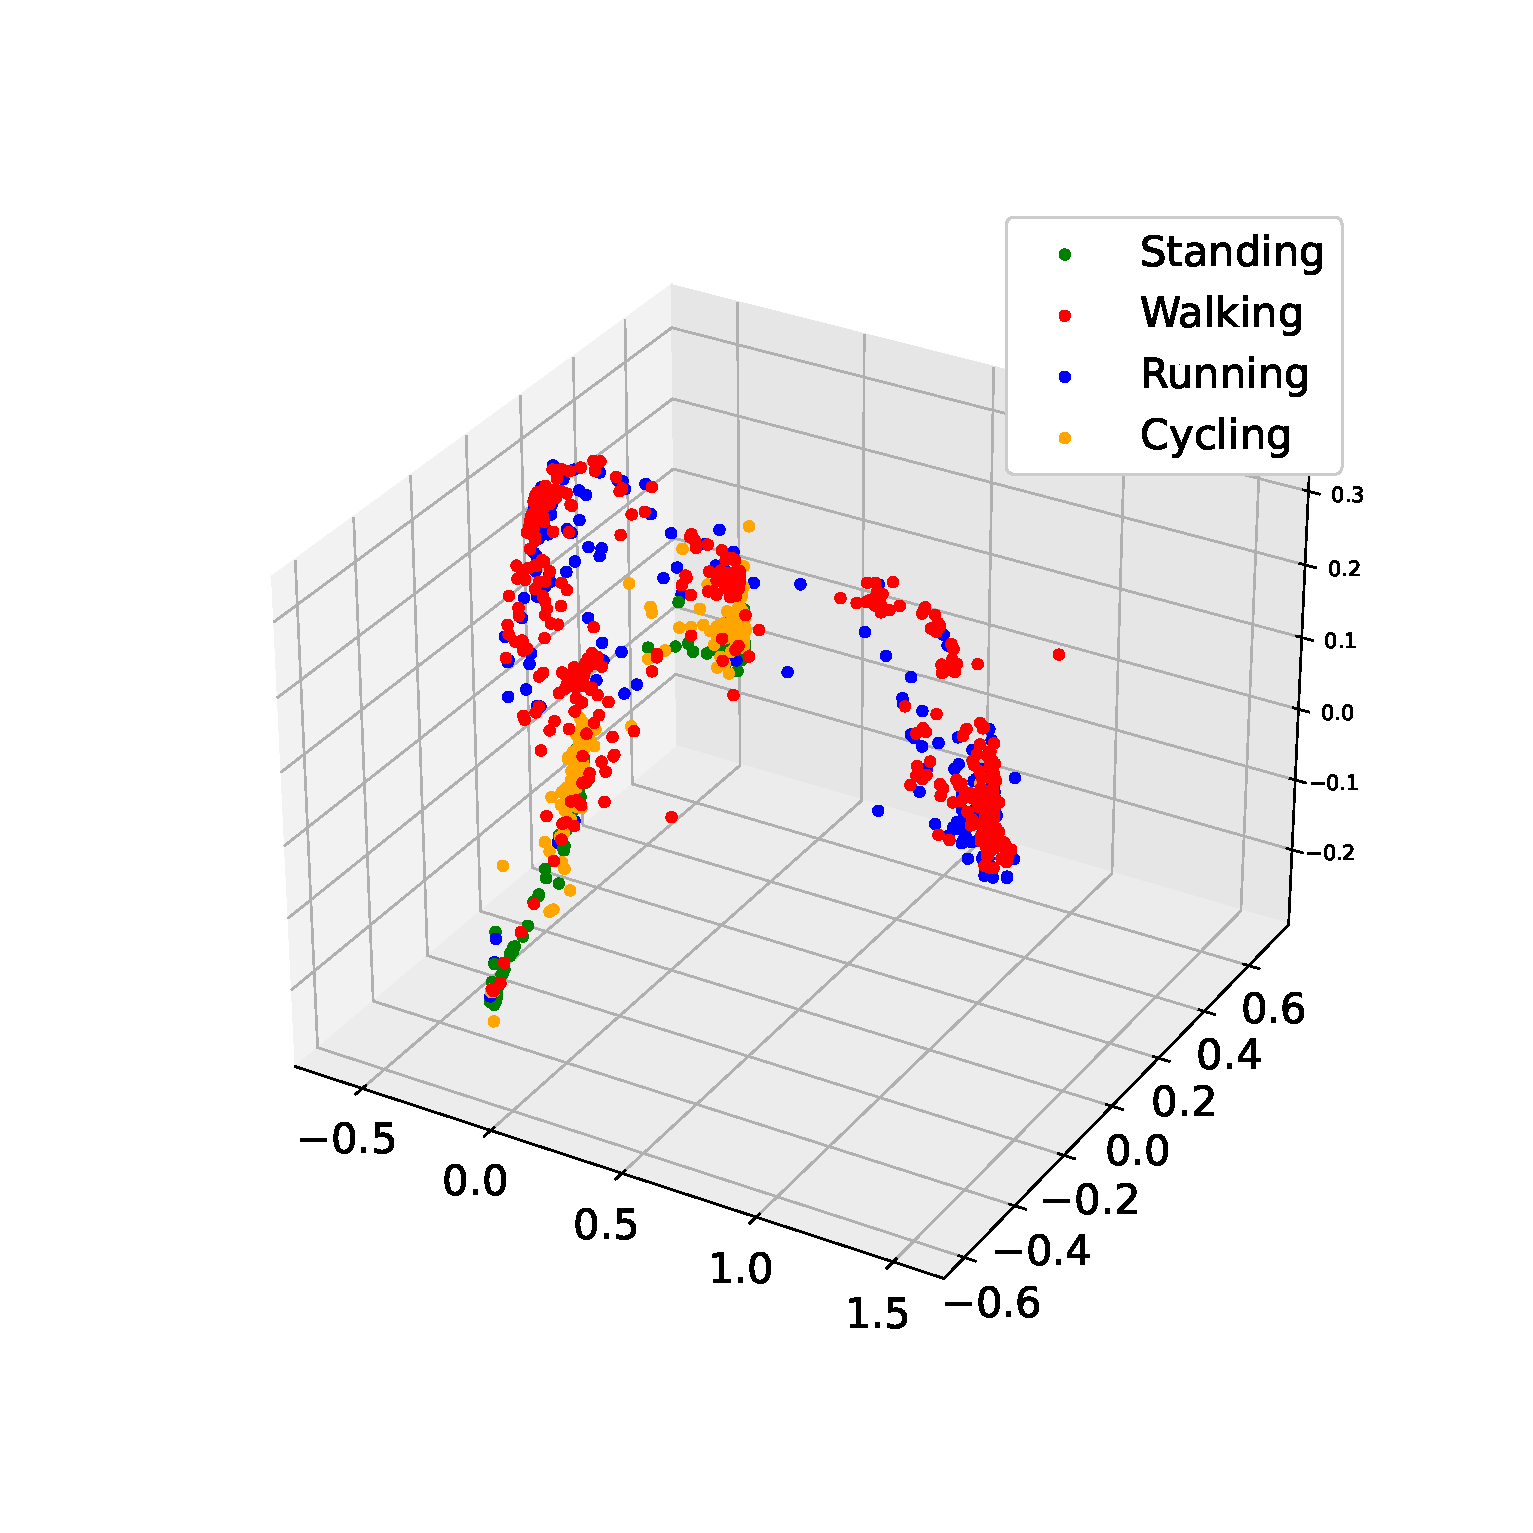
\includegraphics[width=0.6\textwidth]{Data_3D.eps}
                
        \end{columns}

        Accuracy:

        \begin{columns}[c]
        
            \column{0.6\textwidth}
                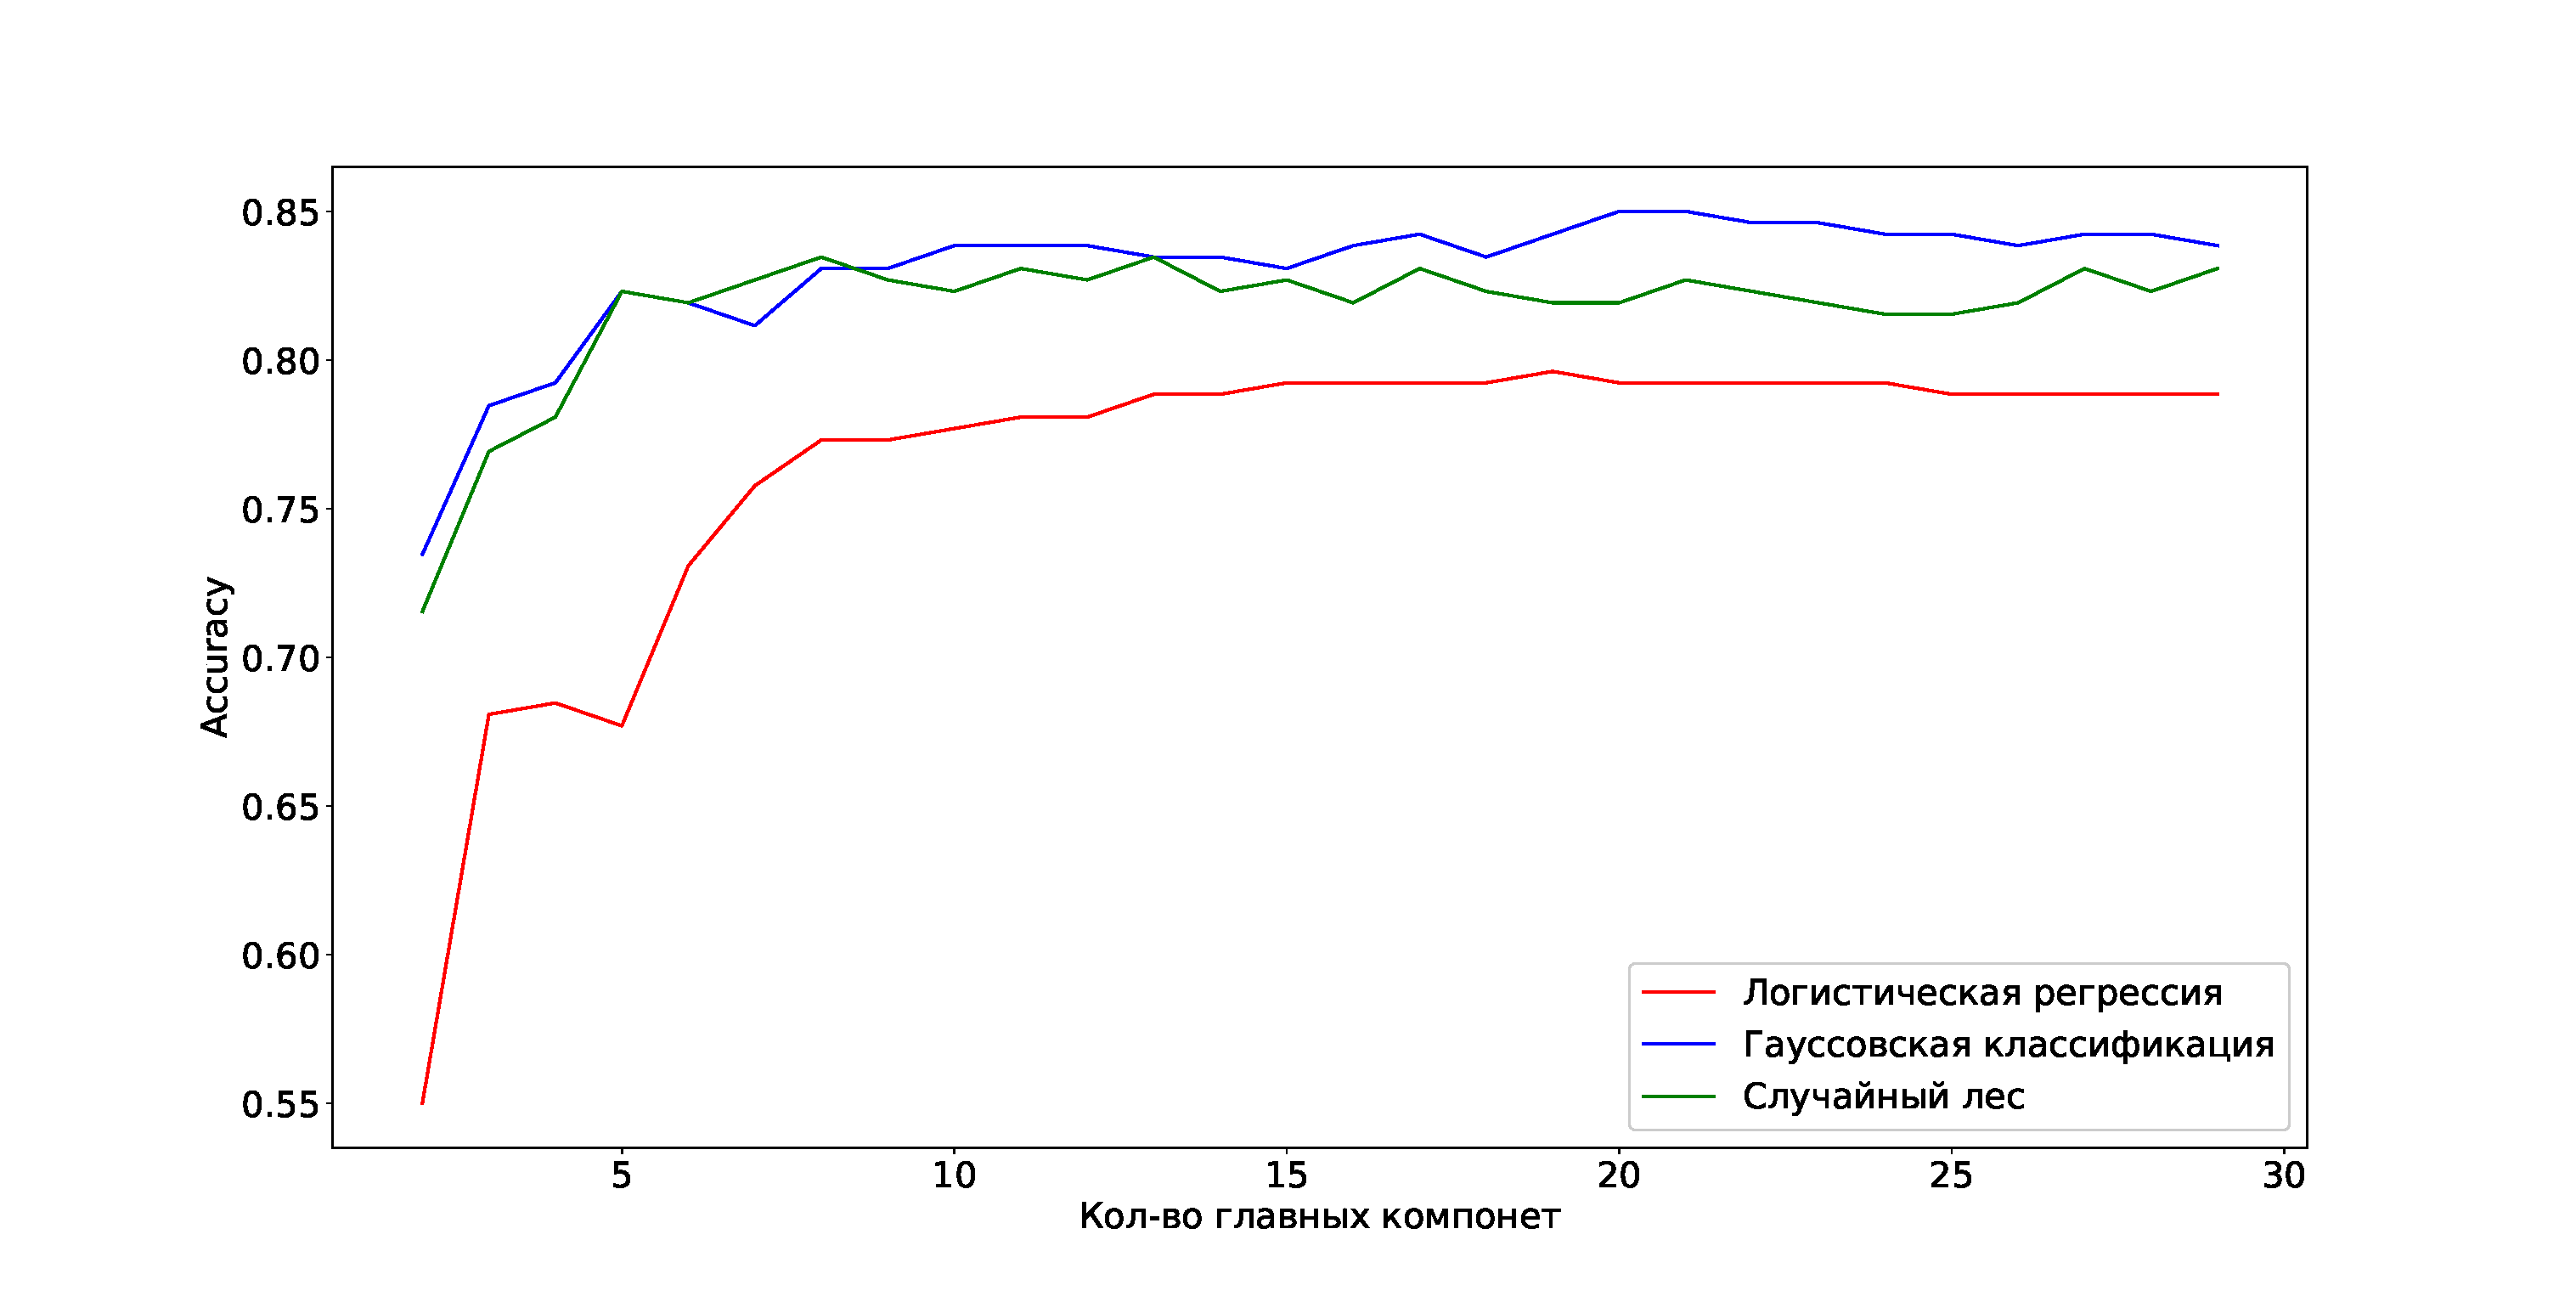
\includegraphics[width=1.1\textwidth]{Accuracy.eps}
                
            \column{0.6\textwidth}
                    \begin{itemize}

                        \item LogisticRegression: 79$\%$

                        \item GaussianProcessClassifier: $86\%$

                        \item RandomForestClassifier: $85\%$

                    \end{itemize}
                
        \end{columns}


\end{frame}

%----------------------------------------------------------------------------------------------------------

\begin{frame}{Заключение}

    \begin{itemize}

        \item Подтверждена гипотеза компактности: векторы параметров, соответствующие траекториям различных классов, оказываются разделимы в своём пространстве.
    
        \item Предложен метод решения задачи классификации динамических систем с помощью лагранжевой нейронной сети.
        
        \item Проведен вычислительный эксперимент на датасате PAMAP2, в которых проведено сравнение различных методов классификации.

    \end{itemize}
    
\end{frame}

%----------------------------------------------------------------------------------------------------------

\begin{frame}{Планы}

    \begin{itemize}

        \item Доделать эксперимент на весь датасет с использованием всех акселерометров и всех классов.
    
        \item Сделать свой датасет.
        
    \end{itemize}
    
\end{frame}

%----------------------------------------------------------------------------------------------------------

\end{document} 